\chapter{Implementierung}
\label{chap:implementierung}

\section{Technologische Basis}
Die Implementierung basiert auf einer sorgfältig ausgewählten technologischen Basis, die modernste Tools und Frameworks kombiniert, um eine effiziente und skalierbare Lösung zu gewährleisten. Die wichtigsten Technologien sind:
\begin{itemize}
    \item \textbf{Frontend:} Entwicklung mit React und TypeScript. Material-UI wird für konsistente UI-Komponenten genutzt, während Vite für schnelle Build- und Entwicklungsprozesse sorgt.
    \item \textbf{Backend:} Aufbau von RESTful APIs mit .NET Core. Middleware-Services ermöglichen Authentifizierung, Fehlerbehandlung und Protokollierung.
    \item \textbf{Datenbank:} Relationale Modellierung und Abfragen in Azure SQL mit Entity Framework Core für nahtlosen Datenzugriff.
    \item \textbf{DevOps:} Automatisierte CI/CD-Pipelines mit Azure Pipelines, die den Entwicklungs- und Bereitstellungsprozess optimieren.
\end{itemize}

\section{Detailierte Architektur}
\subsection{Frontend-Architektur}
Das Frontend wurde mit einer komponentenbasierten Architektur entwickelt, die eine modulare und wiederverwendbare Struktur ermöglicht:
\begin{itemize}
    \item \textbf{Komponenten:} Jedes UI-Element wurde als eigenständige Komponente entwickelt, um Wartbarkeit und Wiederverwendbarkeit zu maximieren.
    \item \textbf{State-Management:} Für die Verwaltung globaler Zustände kommen Redux Toolkit und Zustand zum Einsatz.
    \item \textbf{Datenvisualisierung:} ApexCharts und React-AäpexCharts werden zur Darstellung von Donut- und Radarcharts verwendet.
\end{itemize}

\begin{minted}[linenos, frame=single, fontsize=\small, caption=Beispiel einer React-Komponente, label=lst:react_component]{javascript}
import React from 'react';
import { Chart } from 'react-apexcharts';

const RadarChart = () => {
  const data = {
    labels: ['Teamarbeit', 'Effizienz', 'Pünktlichkeit', 'Innovation'],
    datasets: [
      {
        label: 'Mitarbeiter A',
        data: [80, 90, 70, 85],
        backgroundColor: 'rgba(54, 162, 235, 0.2)',
        borderColor: 'rgba(54, 162, 235, 1)',
        borderWidth: 2,
      },
    ],
  };

  return <Chart options={data} type="radar" />;
};

export default RadarChart;
\end{minted}


\section{Backend-Architektur}
Das Backend basiert auf einer mehrschichtigen Architektur, die eine klare Trennung von Verantwortlichkeiten gewährleistet. Diese Architektur stellt die Grundlage für eine effiziente und skalierbare Verarbeitung von Mitarbeitendengesprächsdaten dar.

\subsection{Technologische Basis}
Die Entwicklung des Backends erfordert eine fundierte Auswahl moderner Technologien und Methoden, um zentrale Anforderungen wie Sicherheit, Performanz, Skalierbarkeit und Datenverarbeitung zu erfüllen. Folgende Komponenten sind integraler Bestandteil der Implementierung:
\begin{itemize}
    \item \textbf{API-Entwicklung:} Implementierung von RESTful APIs mit .NET Core, die eine zuverlässige und standardisierte Datenübertragung ermöglichen.
    \item \textbf{Cloud-Technologien:} Integration von Microsoft Azure-Diensten wie Azure SQL und Azure Service Bus zur Unterstützung asynchroner Kommunikation und Datenverarbeitung.
    \item \textbf{Sicherheitsmechanismen:} Einsatz von Azure Active Directory (AAD) für Multi-Faktor-Authentifizierung und rollenbasierte Zugriffskontrolle.
    \item \textbf{Datenverarbeitung:} Nutzung skalierbarer Algorithmen zur Aggregation und Transformation komplexer Datenstrukturen.
\end{itemize}

\subsection{Komponenten der Backend-Architektur}
\begin{itemize}
    \item \textbf{Controller-Schicht:} Zuständig für die Verarbeitung von Anfragen und das Routing.
    \item \textbf{Service-Schicht:} Implementiert die Geschäftslogik und ist für Datenverarbeitung und Validierung verantwortlich.
    \item \textbf{Repository-Schicht:} Ermöglicht den Zugriff auf die Datenbank mithilfe von Entity Framework Core.
    \item \textbf{Middleware:} Authentifizierung und Fehlerbehandlung werden zentral über Middleware-Komponenten gesteuert.
\end{itemize}

\subsection{API-Endpunkte}
Zur Interaktion mit den Daten des Systems wurden verschiedene API-Endpunkte implementiert. Die folgende Tabelle listet die wesentlichen HTTP-Methoden und URLs zur Manipulation von Ressourcen:

\begin{table}[H]
\caption{HTTP-Methoden und URLs zur Manipulation von Ressourcen}
\label{table:http-methods}
\raggedright
{\scriptsize Quelle: Eigene Darstellung} \\[0.3em]
\renewcommand{\arraystretch}{1.1} % Leichter reduzierter Zeilenabstand
\setlength{\tabcolsep}{1.8pt} % Weiter verringerter horizontaler Zellabstand
\begin{tabularx}{\textwidth}{>{\centering\arraybackslash}m{2cm}|>{\centering\arraybackslash}m{5.5cm}|>{\raggedright\arraybackslash}m{6.5cm}}
\hline
\textbf{HTTP-Methoden} & \textbf{URL /odata/v\{version\}} & \textbf{Beschreibung} \\ \hline
GET & /employeeAppraisals/\{appraisalId\} & Lese ein einzelnes Mitarbeitergespräch anhand der eindeutigen ID, um detaillierte Informationen zu erhalten. \\ \hline
GET & /employeeAppraisals & Lese alle Mitarbeitergespräche zur Analyse und Berichterstellung. \\ \hline
POST & /employeeAppraisals & Erstelle ein neues Mitarbeitergespräch und speichere es im System. \\ \hline
GET & /employeeAppraisals/all & Lese alle verfügbaren Mitarbeitergespräche, einschließlich archivierter Daten. \\ \hline
GET & /employeeAppraisals/last & Lese die zuletzt eingetragenen Mitarbeitergespräche. \\ \hline
POST & /employeeAppraisals/CheckBox & Erstelle oder aktualisiere Checkbox-Daten für Mitarbeitergespräche, z. B. um spezifische Kriterien zu markieren. \\ \hline
\end{tabularx}
\end{table}


\subsection{Beispiel eines Controllers}
Ein Beispiel für einen .NET Core Controller, der die oben genannten Endpunkte implementiert, ist in Listing \ref{lst:dotnet_controller} dargestellt.


%TODO%


\subsection{Sicherheitsmechanismen und Skalierbarkeit}
Die Sicherheitsmechanismen des Backends gewährleisten die Integrität und Vertraulichkeit sensibler Daten. Hierzu zählen:
\begin{itemize}
    \item \textbf{Authentifizierung:} Azure Active Directory ermöglicht Multi-Faktor-Authentifizierung und Single Sign-On.
    \item \textbf{Datenverschlüsselung:} Sensible Daten werden durch AES-256 sowohl im Ruhezustand als auch während der Übertragung geschützt.
    \item \textbf{Rollenbasierte Zugriffskontrolle:} Strikte Zugriffsrichtlinien stellen sicher, dass nur autorisierte Personen auf spezifische Daten zugreifen können.
\end{itemize}

\subsection{Integration von Microsoft Azure-Diensten}
Die Einbindung von Microsoft Azure-Diensten spielt eine zentrale Rolle in der Backend-Entwicklung:
\begin{itemize}
    \item \textbf{Azure SQL:} Bereitstellung einer skalierbaren und sicheren Plattform für die Speicherung großer Mengen sensibler Daten.
    \item \textbf{Azure Service Bus:} Unterstützung asynchroner Kommunikationsprozesse zwischen Systemkomponenten.
    \item \textbf{Automatisierung:} Erstellung automatisierter Berichte und datenbasierter Einblicke aus den gespeicherten Gesprächsdaten.
\end{itemize}

\subsection{Optimierung der Datenverarbeitung}
Durch die Implementierung moderner Algorithmen wird die Verarbeitung komplexer Datenstrukturen optimiert:
\begin{itemize}
    \item \textbf{Natural Language Processing (NLP):} Analyse unstrukturierter Gesprächsnotizen zur Erkennung von Mustern und Trends.
    \item \textbf{Datenaggregation:} Konsolidierung unterschiedlicher Quellen zur Erstellung ganzheitlicher Analysen.
\end{itemize}

\subsection{Überwachung und Wartbarkeit}
Eine modulare Architektur unterstützt die Wartbarkeit und Überwachung des Systems:
\begin{itemize}
    \item \textbf{Monitoring:} Ein spezifisches Monitoring-System identifiziert Leistungseinbußen und sendet Warnmeldungen.
    \item \textbf{Containerisierung:} Verwendung von Docker, um Konsistenz zwischen Entwicklungs- und Produktionsumgebungen sicherzustellen.
\end{itemize}

\subsection{Zusammenfassung}
Die Backend-Entwicklung kombiniert moderne Technologien und Sicherheitsmechanismen, um eine leistungsfähige, skalierbare und sichere Plattform zur Visualisierung von Mitarbeitendengesprächsdaten bereitzustellen. Durch die Integration von Cloud-Diensten, robusten Algorithmen und einer modularen Architektur wird eine optimale Nutzererfahrung gewährleistet.


\subsection{Datenbankmodell}
Die relationale Datenbank wurde mit Azure SQL implementiert. Wichtige Tabellen und deren Beziehungen sind in Abbildung~\ref{fig:db_er_model} dargestellt. Das Schema wurde so gestaltet, dass es sowohl aktuelle als auch historische Daten effizient speichern kann.

\begin{figure}[h!]
    \centering
    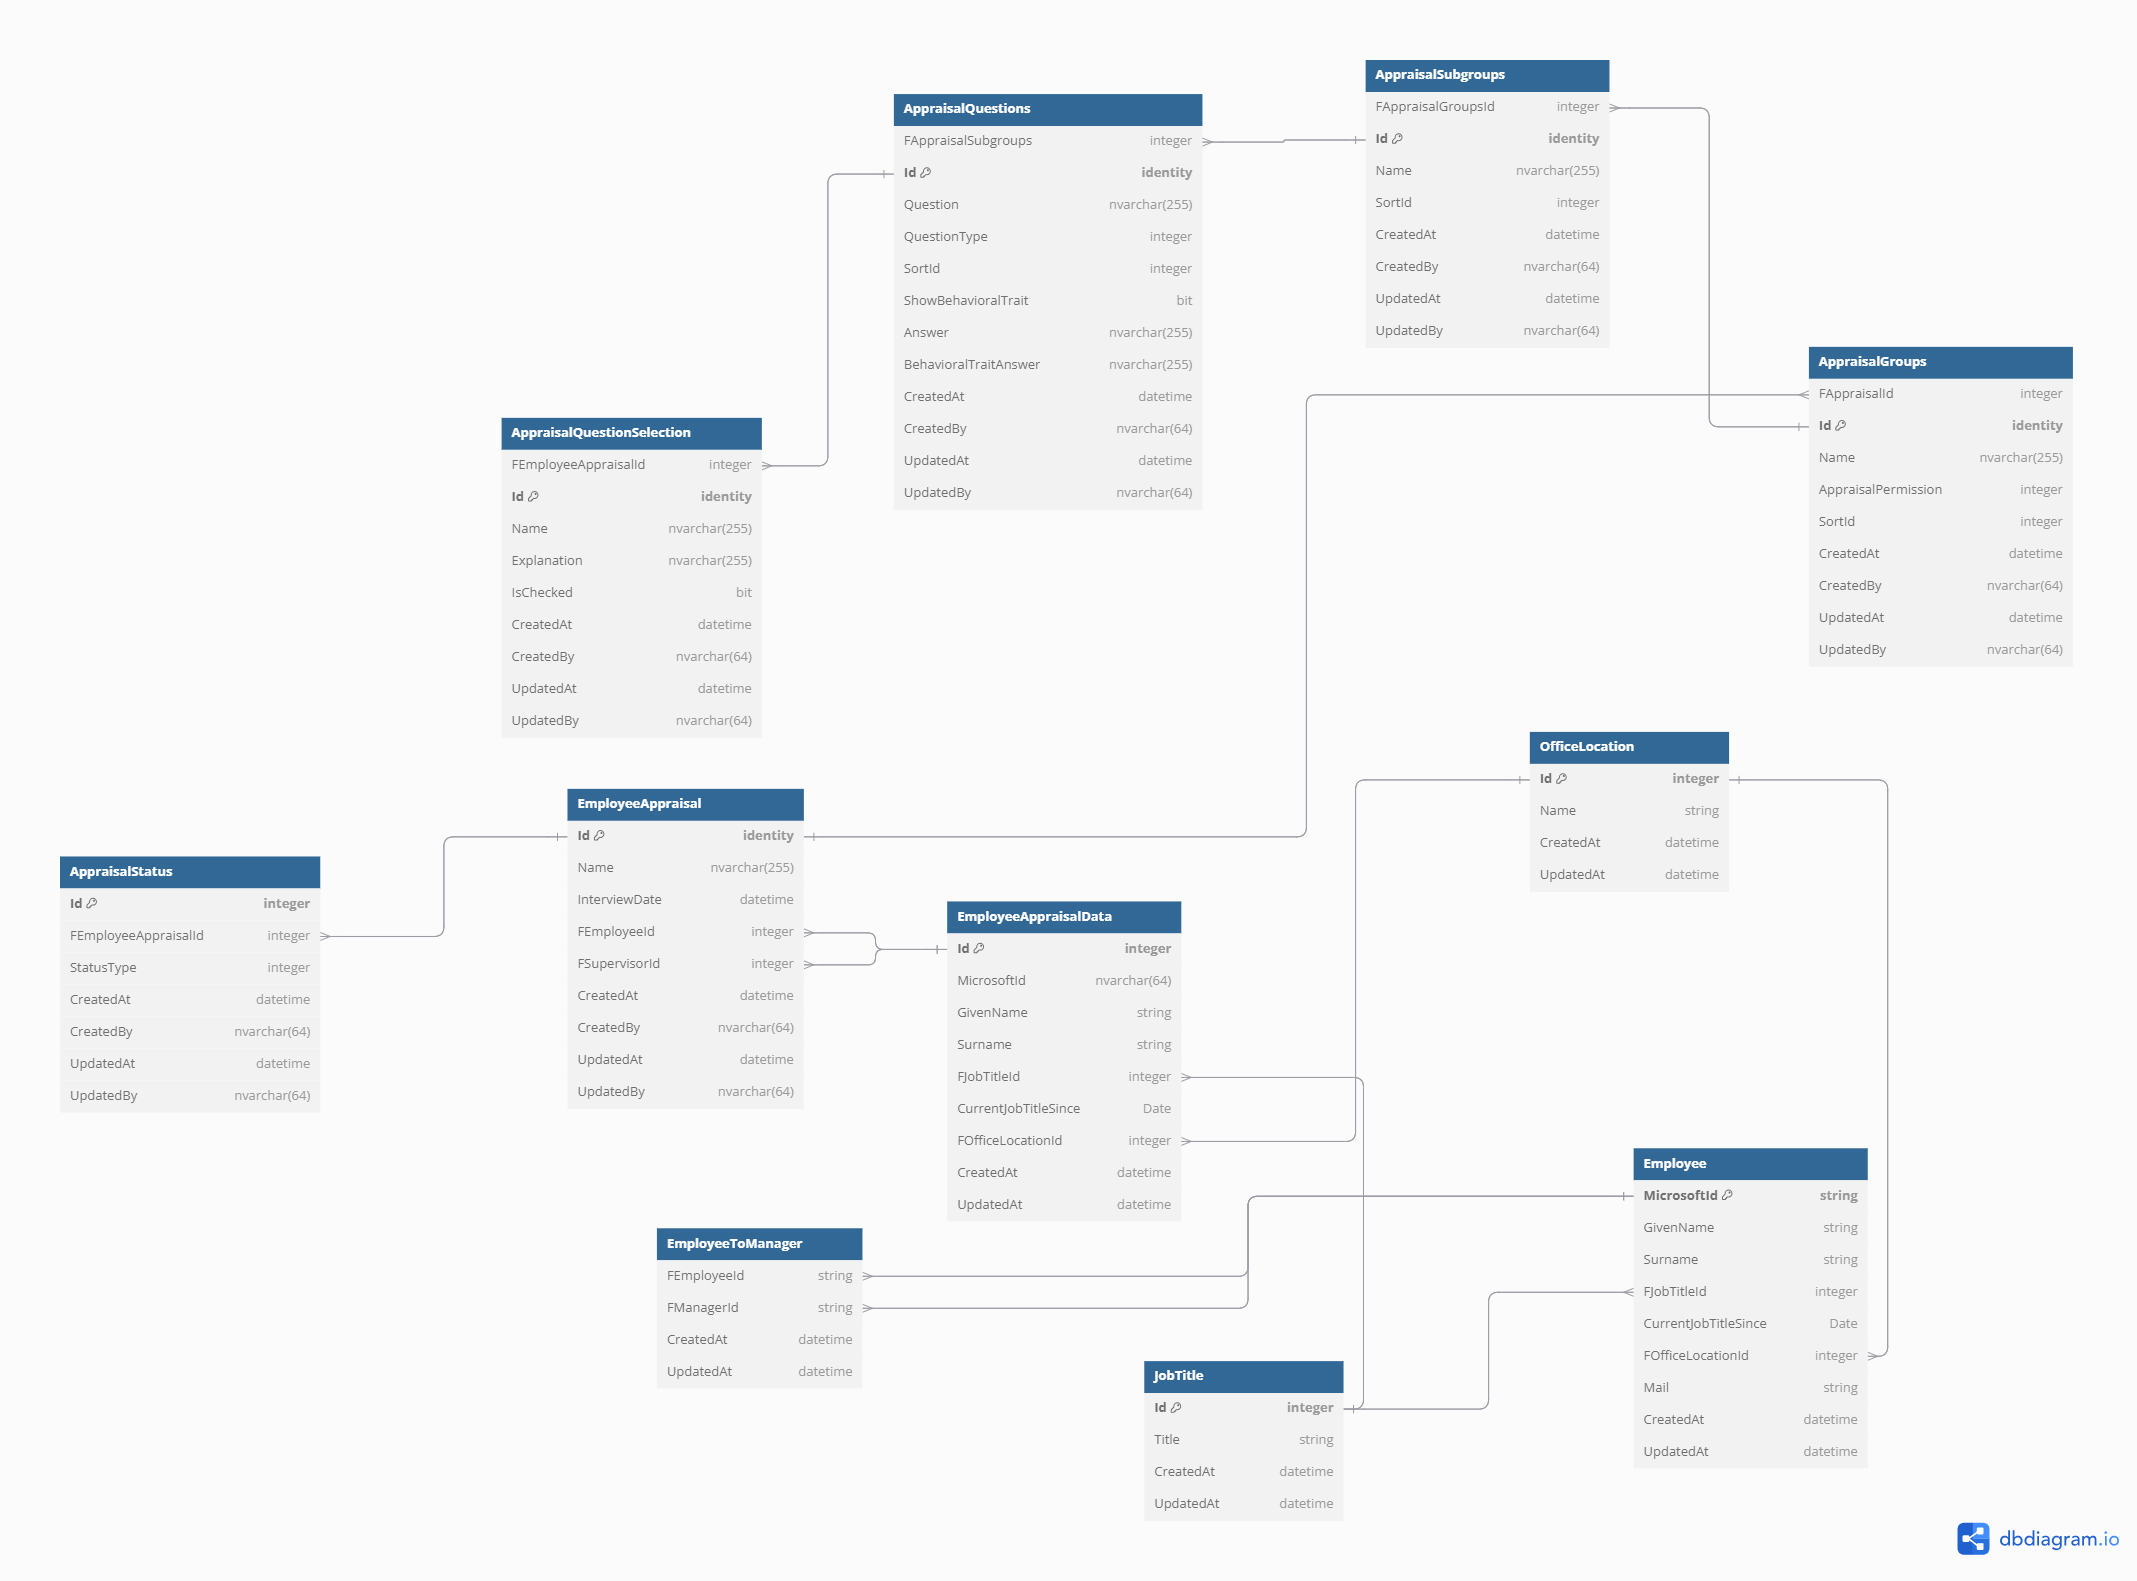
\includegraphics[width=0.8\textwidth]{images/er_modell_design.png}
    \caption{ER-Diagramm der Datenbankstruktur.}
    \label{fig:db_er_model}
\end{figure}

\subsection{Fehleranalyse und Herausforderungen während der Implementierung}
Während der Implementierung traten verschiedene Herausforderungen und Fehler auf, die den Entwicklungsprozess beeinflussten. Diese Probleme wurden systematisch analysiert und durch passende Lösungen behoben:
\begin{itemize}
    \item \textbf{Problem mit Datenkonsistenz:} Bei parallelen Datenbankoperationen traten Inkonsistenzen in den gespeicherten Daten auf. \\
    \textbf{Lösung:} Einführung einer Transaktionsverwaltung im Backend mit Entity Framework Core.
    
    \item \textbf{Middleware-Konflikte:} Fehler in der Middleware-Konfiguration führten zu unerwarteten API-Antworten. \\
    \textbf{Lösung:} Erstellung detaillierter Tests für die Middleware-Komponenten und verbesserte Fehlerbehandlung.

    \item \textbf{Performance-Probleme:} Bei Abfragen großer Datensätze kam es zu erheblichen Verzögerungen. \\
    \textbf{Lösung:} Optimierung der SQL-Abfragen und Implementierung von Indizes zur Verbesserung der Abfragegeschwindigkeit.
\end{itemize}


\section{Herausforderungen und Lösungen}
\subsection{Datenkonsistenz}
Um die Konsistenz der Daten zu gewährleisten, wurde eine Transaktionsverwaltung implementiert. Dies verhindert Dateninkonsistenzen bei parallelen Datenbankoperationen.

\subsection{Echtzeit-Updates}
Mit Azure Service Bus wurde eine asynchrone Kommunikation ermöglicht. Dies erlaubt Echtzeit-Benachrichtigungen an Benutzer, ohne die Backend-Leistung zu beeinträchtigen.

\subsection{Optimierung der Benutzerfreundlichkeit}
Durch regelmäßige Usability-Tests und die iterative Anpassung der UI-Elemente wurde die Benutzerfreundlichkeit kontinuierlich verbessert.

\section{Test- und Debugging-Prozesse}
\subsection{Frontend-Tests}
Komponenten wurden mit Jest und React Testing Library getestet, um deren Funktionalität und Robustheit sicherzustellen.

\subsection{Backend-Tests}
Die RESTful APIs wurden mit Postman und automatisierten Integrationstests getestet.

\subsection{Debugging}
Entwicklerwerkzeuge wie Visual Studio Debugger und Browser DevTools wurden für die Analyse und Behebung von Fehlern verwendet.

\section{Zusammenfassung}
Die Implementierung des Systems kombiniert moderne Technologien, robuste Sicherheitsmaßnahmen und optimierte Workflows. Es bietet eine performante, skalierbare und benutzerfreundliche Lösung, die den Anforderungen moderner HR-Tools gerecht wird.
